\subsection{Предел последовательности}

\begin{definition}
    Окрестность точки $A$: $U_{\eps}(A) = (A - \eps; A + \eps)$
\end{definition}

\begin{figure}[h]
  \centering
  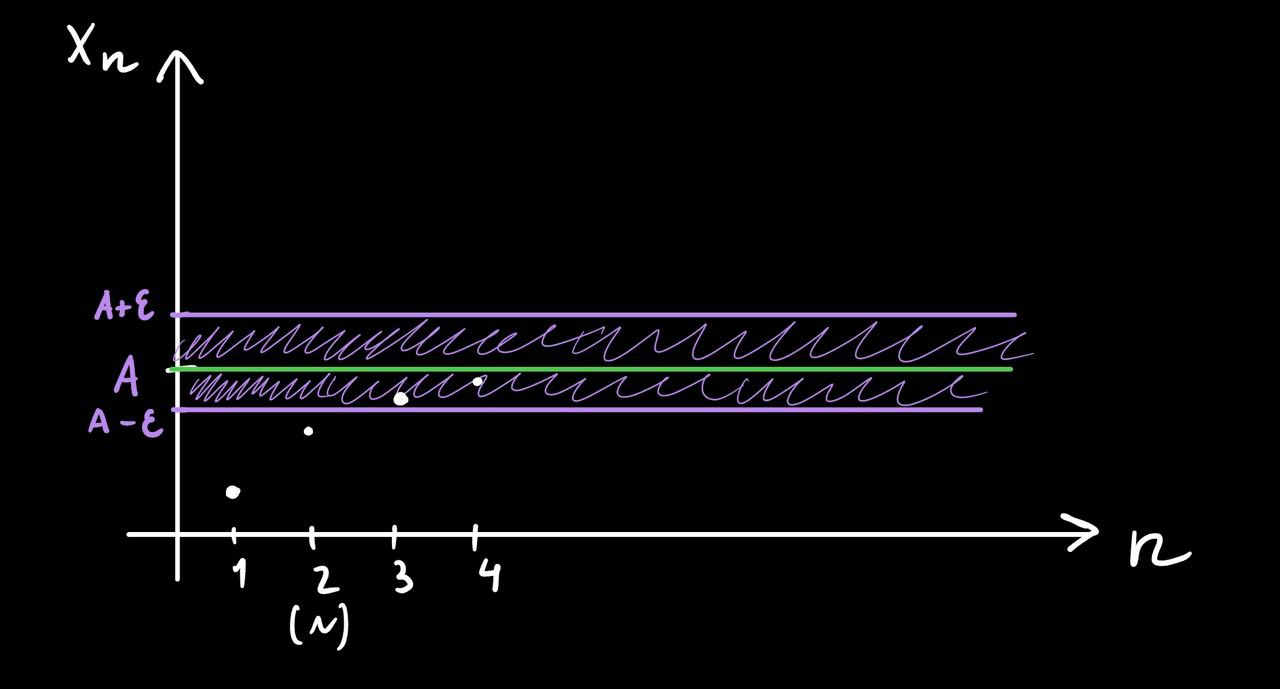
\includegraphics[width=0.8\textwidth]{lectures/files/lec_3_19.09.2025-13-56-05.png}
  \label{fig:lec_3_19.09.2025-13-56-05.png}
\end{figure}

\begin{definition}
    $\Lim{n}{\infty} a_n = A$, если 
    $$\fbox{$ \forall \eps > 0\ \exists N \in \N\ \forall n > N\ |a_n - A| < \eps $}$$
    $$ \Updownarrow $$
    $$ \forall \eps > 0\ \exists N \in \N\ \forall n > N\ -\eps < a_n - A < \eps $$
    $$ \Updownarrow $$
    $$ \forall \eps > 0\ \exists N \in \N\ \forall n > N\ A-\eps < a_n < A+\eps $$
    $$ \Updownarrow $$
    $$ \forall \eps > 0\ \exists N \in \N\ \forall n > N\ a_n \in U_\eps(A) $$
\end{definition}

\begin{example}
    Доказать, что
    $ \Lim{n}{\infty} \frac{1}{n} = 0 $

    $$ \forall \eps > 0\ \exists N \in \N\ \forall n > N\ \l|\frac{1}{n} - 0\r| < \eps $$
    $$ \frac{1}{n} < \eps $$
    $$ n > \frac{1}{\eps} $$
    $$ N(\eps) = \l\lceil \frac{1}{\eps} + 1 \r\rceil $$
\end{example}

\begin{definition}
    Последовательность называется \textbf{сходящейся}, если у нее есть предел 
    $$ \Updownarrow $$
    $$ \exists a : \Lim{n}{\infty} a_n = A $$
\end{definition}

\newpage

\subsection{Теорема об ограниченности сходящейся последовательности}
\begin{theorem}
    Если последовательность сходящаяся, то она ограничена
\end{theorem}
\begin{Proof}
    Рассмотрим $\{a_n\}$
    $$ \exists A\ \forall \eps > 0\ \exists N \in \N\ \forall n > N\ |a_n - A| < \eps $$
    $$ \exists A\ \exists N(1) \in \N\ \forall n > N(1)\ |a_n - A| < 1 \Leftrightarrow a_n \in U_1(A) $$
    Очевидно, что элементов $a_k,\ $где $ k <= N(1)$ конечное число. А для всех элементов $a_n,\ n > N(1)$ выполняется $|a_n - A| < 1$. Тогда можем взять нижнюю границу $min\{a_1,\ldots,a_{N(1)}, A-1\}$ и верхнюю $max\{a_1,\ldots,a_{N(1)}, A+1\}$.
\end{Proof}

\begin{figure}[h]
  \centering
  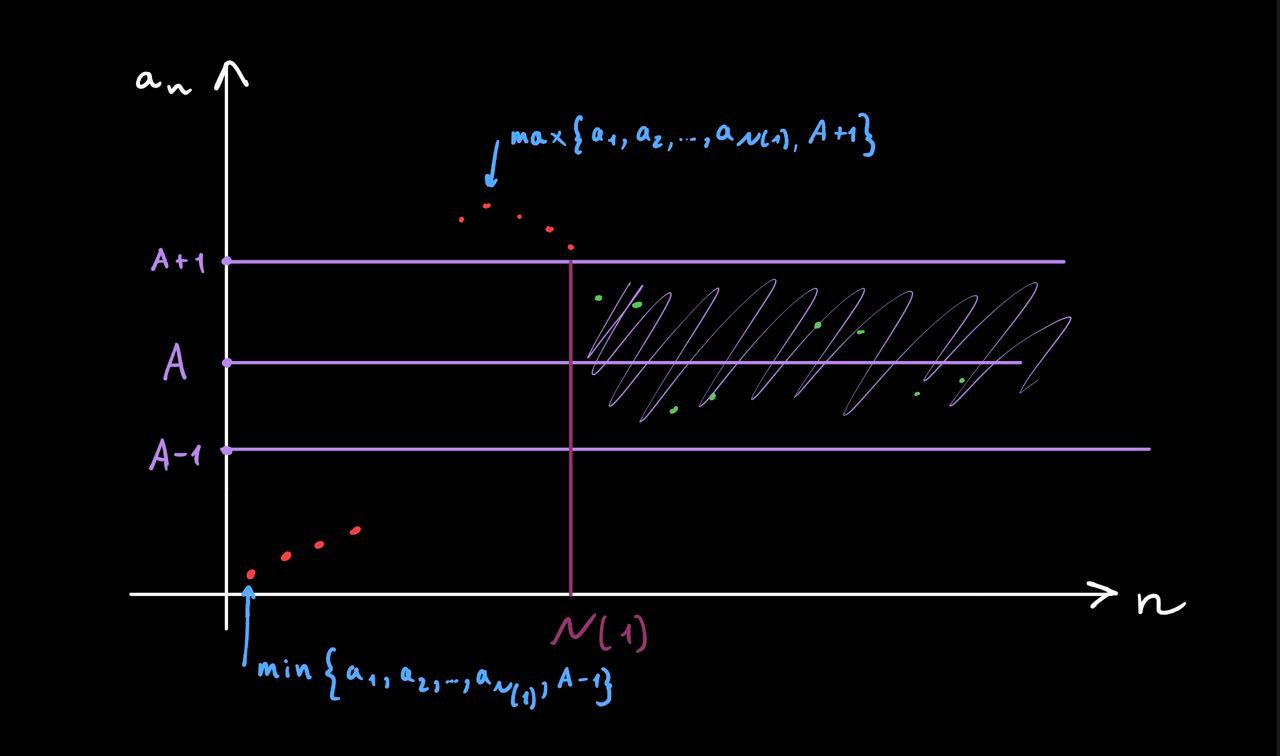
\includegraphics[width=0.8\textwidth]{lectures/files/lec_3_19.09.2025-14-15-52.png}
  \caption{К доказательству}
  \label{fig:lec_3_19.09.2025-14-15-52.png}
\end{figure}

\begin{theorem}
    У последовательности может быть только 1 предел
\end{theorem}

\begin{Proof}
    Пп $\exists$ хотя бы 2 lim : $A$ и $B$, $A \neq B$
    $$ \forall \eps > 0\ \exists N_1(\eps) \in \N\ \forall n > N_1(\eps)\ a_n \in U_{\eps}(A) $$
    $$ \forall \eps > 0\ \exists N_2(\eps) \in \N\ \forall n > N_2(\eps)\ a_n \in U_{\eps}(B) $$
    Возьмем $\eps_0 = \frac{|A - B|}{3}$ и $n_0 = N_1(\eps_0) + N_2(\eps_0) $

    Получаем
    $$ a_{n_0} \in U_{\eps_0}(A),\ a_{n_0} \in U_{\eps_0}(B) $$
    Но 
    $$ U_{\eps_0}(A) \cap U_{\eps_0}(B) = \varnothing $$
    Противоречие
\end{Proof}

\subsection{Арифметика предела}
$ \Lim{n}{\infty}a_n = A $, $ \Lim{n}{\infty}b_n = B $, то

\begin{itemize}
    \item[1)] $\Lim{n}{\infty}(a_n + b_n) = A + B$
    \item[2)] $\Lim{n}{\infty}(a_n \cdot b_n) = A \cdot B$
    \item[3)] $\Lim{n}{\infty}\frac{a_n}{b_n} = \frac{A}{B}$ $(b_n \neq 0; B \neq 0)$
    \item[4)] $\Lim{n}{\infty}\sqrt{a_n} = \sqrt{A}$ $(a_n \geq 0; A \geq 0)$
\end{itemize}

\begin{Proof}[Доказательство свойства 1]
    $$ \forall \eps > 0\ \exists N_1(\eps) \in \N\ \forall n > N_1(\eps)\ |a_n - A| < \eps $$
    $$ \forall \eps > 0\ \exists N_2(\eps) \in \N\ \forall n > N_2(\eps)\ |b_n - B| < \eps $$
    Хотим
    $$ \forall \eps > 0\ \exists N_3(\eps) \in \N\ \forall n > N_3(\eps)\ |(a_n + b_n) - (A + B)| < \eps $$
    $$\Updownarrow$$
    $$ \forall \eps > 0\ \exists N_3(\eps) \in \N\ \forall n > N_3(\eps)\ |(a_n - A) + (b_n - B)| < \eps $$
    $$\Uparrow$$
    $$ \forall \eps > 0\ \exists N_3(\eps) \in \N\ \forall n > N_3(\eps)\ \underbrace{|a_n - A|}_{< \frac{\eps}{3}} + \underbrace{|b_n - B|}_{< \frac{2\eps}{3}} < \eps $$
    $$ \forall n > N_1\l(\frac{\eps}{3}\r)\ \forall n > N_2\l(\frac{2\eps}{3}\r)$$
    $$ N_3(\eps) = max\l\{N_1\l(\frac{\eps}{3}\r), N_2\l(\frac{2\eps}{3}\r)\r\}$$
\end{Proof}

Примечание: Доказательства свойств 2 и 3, рассмотренные далее, были выведены после доказательства теоремы о произведении б.м. и огр. последовательностей

\begin{Proof}[Доказательство свойства 2]
    Хотим
    $$\Lim{n}{\infty}(a_n \cdot b_n) = A \cdot B$$
    По теореме о связи предела с бесконечно малой последовательностью
    $$ \alpha_n=(a_n - A) \text{ --- б.м.} ,\ \beta_n=(b_n - B) \text{ --- б.м.} $$
    Хотим
    $$ (a_n b_n - AB) \text{~--- б.м.} $$
    $$ (a_n b_n - AB) = (\alpha_n + A)(\beta_n + B) - AB = \alpha_n\beta_n + \alpha_nB + A\beta_n + AB - AB = $$
    $$ =\underbrace{\alpha_n\beta_n}_{\text{б.м.}} + \underbrace{\alpha_nB}_{\text{б.м.}} + \underbrace{\underbrace{A}_{\text{огр}}\underbrace{\beta_n}_{\text{б.м.}}}_{\text{б.м.}} = \text{б.м.} + \text{б.м.} + \text{б.м.} = \text{б.м.}$$
\end{Proof}

\begin{Proof}[Доказательство свойства 3]
    Хотим 
    $$\Lim{n}{\infty}\frac{a_n}{b_n} = \frac{A}{B}\ (b_n \neq 0; B \neq 0)$$
    По теореме о связи предела с бесконечно малой последовательностью
    $$ \alpha_n=(a_n - A) \text{ --- б.м.} ,\ \beta_n=(b_n - B) \text{ --- б.м.} $$
    Хотим
    $$ \frac{a_n}{b_n} - \frac{A}{B} \text{ --- б.м.} $$
    $$ \frac{a_n}{b_n} - \frac{A}{B} = \frac{\alpha_n + A}{\beta_n + B} - \frac{A}{B} = \frac{(\alpha_n + A)B - A(\beta_n + B)}{(\beta_n + B)B} = $$
    $$ = \frac{(\alpha_n + A)B - A(\beta_n + B)}{(\beta_n + B)B} = \frac{\alpha_nB + AB - A\beta_n - AB}{b_nB} = \frac{\alpha_nB - A\beta_n}{b_nB} = $$
    $$ = \underbrace{\frac{1}{b_n} \cdot \frac{1}{B}}_{\text{огр $\cdot$ огр}} \cdot \underbrace{(\alpha_nB - A\beta_n)}_{\text{б.м}} = \text{б.м.} $$

\end{Proof}

\subsection{Бесконечно большая и бесконечно малая последовательности}

\begin{definition}
    \textbf{Бесконечно малой} (б.м.) последовательностью называют последовательность $\{a_n\}_{n\in\N}$ такую что, $ \Lim{n}{\infty} a_n = 0 $
\end{definition}

\begin{definition}
    \textbf{Бесконечно большой} (б.б.) последовательностью называют последовательность $\{b_n\}_{n\in\N}$ такую что, $ \Lim{n}{\infty} b_n = \infty $

    $$ \forall M > 0\ \exists N(M) \in \N\ \forall n > N(M)\ |b_n| > M $$
    $$ b_n > M\ (+ \infty) $$
    $$ b_n < M\ (- \infty) $$
\end{definition}

\begin{theorem}
    $$\frac{1}{\text{б.б.}} = \text{б.м.}$$
\end{theorem}

\begin{Proof}
    Пусть $b_n$ - б.б. Тогда
    $$ \forall M > 0\ \exists N_1(M) \in \N\ \forall n > N_1(M)\ |b_n| > M $$
    Хотим $a_n = \frac{1}{b_n}$ - б.м.:
    $$ \forall \eps > 0\ \exists N_2(\eps)\ \forall n > N_2(\eps)\ |a_n| < \eps $$
    $$ \l|\frac{1}{b_n}\r| < \eps $$
    $$ \l|b_n\r| > \frac{1}{\eps} $$
    Возьмем $N_2(\eps) = N_1\l(\frac{1}{\eps}\r) + 1$
\end{Proof}

\begin{theorem}
    \center{б.м. $\cdot$ огр. = б.м.}
\end{theorem}

\begin{Proof}
    Хотим $ a_n \cdot b_n = c_n $, где $a_n, c_n$ - б.м., $b_n$ - огр.

    $$ \forall \eps > 0\ \exists N_1(\eps) \in \N\ \forall n > N_1(\eps)\ |a_n| < \eps $$
    $$ \exists c\ \forall n \in \N\ |b_n| \leq c $$
    Хотим:
    $$ \forall \eps > 0\ \exists N_2(\eps) \in \N\ \forall n > N_2(\eps)\ |a_n \cdot b_n| < \eps $$
    $$ \Uparrow $$
    $$ |a_n| \cdot |b_n| < \eps $$
    $$ |a_n| \cdot c < \eps $$
    $$ |a_n| < \frac{\eps}{c} $$

    Возьмем $N_2(\eps) = N_1\l(\frac{\eps}{c}\r)$
\end{Proof}
